


\section{Description of regulatory network}\label{sec:litrev:theme2}

In figure \ref{fig:circuit}, we present a simplified gene regulatory network that describes the interactions
between the master regulator Spo0A, and the biofilm regulatory proteins SinI, SinR, and SlrR.

Surfactin is known to indirectly activate the expression of genes that produce matrix,
 although the precise molecular process is not fully understood. It has been suggested that 
 surfactin creates pores in the membrane, leading to the leakage of potassium ions from the cytoplasm
  to the outside of the cell. This causes the activation of the membrane sensor kinase KinC when potassium 
  levels are low, which then phosphorylates the master gene regulator Spo0A{\footnotesize\cite{Lpez20091}}. However, some studies contradict this exact mechanism.{\footnotesize\cite{Devi2015}}
Another mechanism responsible for indirectly activating the matrix-producing genes
is nutrient depletion, by which kinases (such as KinA) phosphorylate Spo0A, which is can then 
activate the transcription of SinI.

When Spo0A is activated (phosphorilated), it triggers the transcription of the SinI protein. The SinI protein binds to the SinR protein to form a SinI-SinR complex, which effectively titrates SinR, reducing the number of freely available SinR proteins. SinR is a protein that suppresses the transcription of genes related to matrix production. By disabling SinR through the formation of the SinI-SinR complex, the cell can activate the genes responsible for matrix production.{\footnotesize\cite{Chai2011}}

Furthermore, SinR also inhibits the expression of another protein known as SlrR. If SlrR is expressed, it can also suppress SinR by interacting with it to form a SlrR-SinR complex.{\footnotesize\cite{Chai2011}}

Spo0A has a self-regulatory mechanism that allows it to activate or repress its own transcription
depending on the concentration of its phosphorylated form.
 When Spo0A$\sim$P is absent, the gene \textit{spo0A} is transcribed at a basal low-rate during vegetative growth; 
 this transcription is mediated by the housekeeping sigma factor \(\sigma^A\) and the promoter \textit{$P_V$}.
 At non-zero low concentrations of Spo0A$\sim$P, the transcription of \textit{spo0A} is further activated
 with the help of the \textit{$P_S$} promoter and the \(\sigma^H\) factor. At these low concentrations, Spo0A$\sim$P activates
 biofilm formation and the expression of toxins involved in cannibalism. If the concentration of Spo0A$\sim$P increases further, 
 it will reach high levels, which will lead to the repression of the \textit{spo0A} gene and \textit{sinI} gene
 transcription, while activating the transcription of genes responsible for sporulation.

\begin{figure}[h]
    \centering
    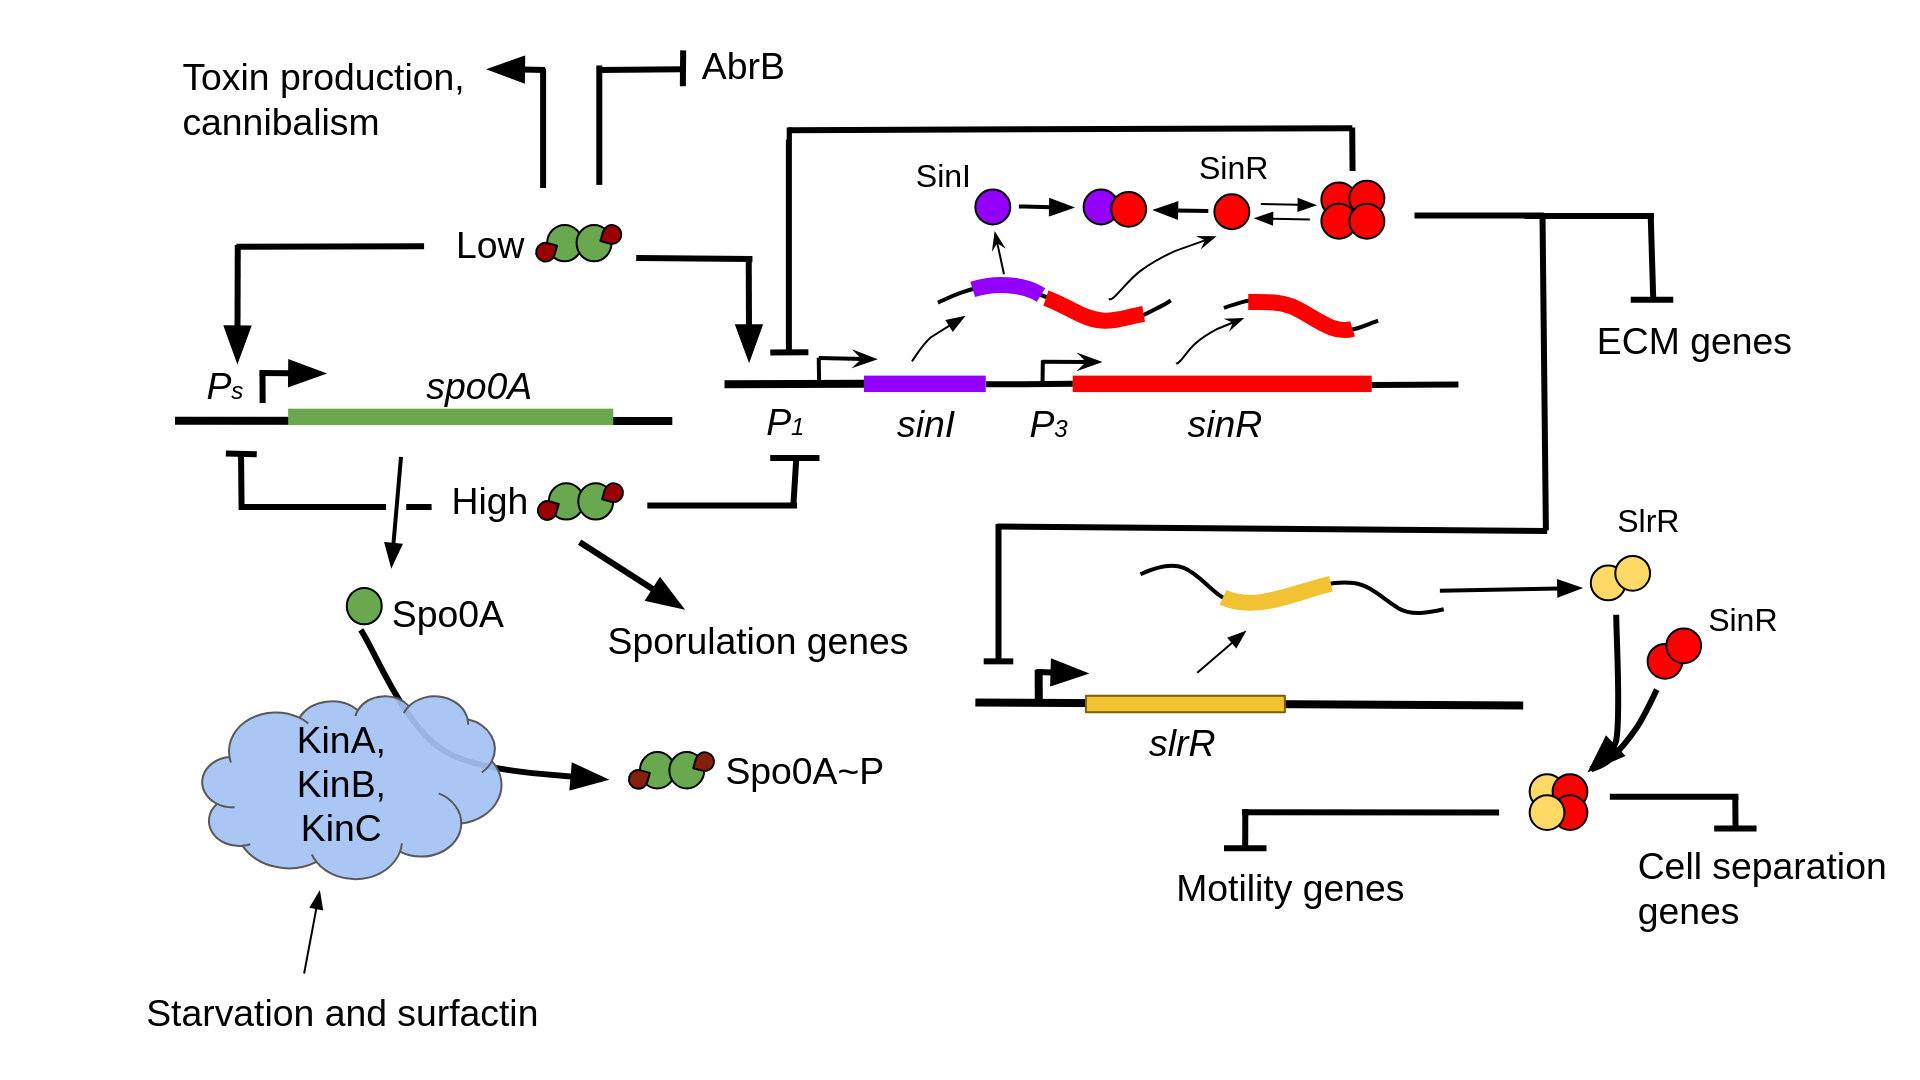
\includegraphics[width=0.8\textwidth]{figures/circuit.png}
    \caption{Gene regulatory network of genes involved in biofilm formation (sinI, sinR, slrR), sporulation (spo0A), and cannibalism.
    }
    \label{fig:circuit}
\end{figure}


\section{Mathematical modelling}\label{sec:litrev:theme2}
Several authors have formulated systems of differential equations to quantitatively model the biomolecular dynamics involved in the gene regulatory network that controls the expression of the extracellular matrix. The systems of equations describe the changes in the concentration of SinR, SinI, and SlrR proteins in the cytoplasm of individual \textit{Bacillus subtilis} cells over time.{\footnotesize\cite{simon}\cite{Voigt2005}\cite{Newman2013}\cite{Chen2023}\cite{Pedreira2021}\cite{Hallinan2010}}. Having considered the models proposed by these authors, we have decided to adopt a modified version of the model proposed by Dannenberg et al. {\footnotesize\cite{simon}} as the basis for our own model. The model is described by the following system of differential equations:

\begin{align}
\frac{dR}{dt} &= P_{1}g(R)f(A)+P_{3} - K_{on(RI)} R I - K_{on(RL)}RL  - D_{R} R, \label{eq:1} \\
\frac{dI}{dt} &= P_{1}g(R)f(A)  - K_{on(RI)} R I - D_{I} I, \label{eq:2} \\
\frac{dL}{dt} &= P_{L}g(R) - K_{on(RL)} RL - D_{L} L , \label{eq:3} \\
\frac{dA}{dt} &= P_V + P_S f(A_p) - D_A A - K_{p}A S , \label{eq:4} \\
\frac{dA_p}{dt} &= K_{p}A S - D_A A_p, \label{eq:5}
\end{align}

where  \(P_V\) and \(P_S\) represent the basal and activated production rates of Spo0A, respectively.
\(P_3\), \(P_1\), and \(P_L\) represent the 
 production rates of SinR, SinI and SlrR due to the activation of their corresponding promoters.
 \(R\), \(I\), \(L\), and \(A\) represent the protein concentrations of SinR, SinI, SlrR, and Spo0A$\sim$P within a single
  bacterial cell. \(K_{on(XY)}\) represents the rate constant for the formation of the $(XY)$ complex,
   while \(D_Z\) encompasses both the dilution rate of component $Z$ caused by cell
    growth and the degradation rate caused by protein breakdown. The phenomenological 
    Haldane equation \(f(A)\) and the repression Hill function \(g(R)\) are defined as follows:


\begin{align*}
    f(A_p) &= \left(\frac{(A_p/K_A)}{1 + (A_p/K_A)+ \frac{A_p^2}{K_A K_S }} \right) \\ 
    g(R) &= \left(\frac{1}{1 + (R/K_R)}\right) \\
\end{align*}  

where $A$ represents the concentration of Spo0A$\sim$P in the cytoplasm. \(K_{A}\) and \(K_R\) represent
 the binding affinities of Spo0A and SinR, respectively, while \(n_A\) and \(n_R\) represent 
 the cooperativities of the binding. \(K_S\) is a constant that accounts for the inhibition of Spo0A$\sim$P 
 when it reaches high concentrations.

Equation (\ref{eq:1}) describes the dynamics of the SinR protein concentration in the cell. SinR is 
produced at a basal rate $P_3$, but its concentration is reduced by a combination of degradation and dilution 
at a rate $D_R$ due to cell growth, or 
increased by the activation mediated by low levels of Spo0A$\sim$P.
Additionally, the concentration of SinR is affected by its interaction with SinI and SlrR, which form complexes with SinR at rates $K_{on(RI)}$ and $K_{on(RL)}$, respectively, leading to a reduction in free SinR molecules.

Equation (\ref{eq:2}) represents the changes in the concentration of SinI. SinI is produced according to its own maximum production rate $P_1$, which is modulated by the function $g(R)$ that models SinR's repression, and the
 function $f(A)$ which accounts for activation by low levels of Spo0A$\sim$P and repression by high 
 levels of Spo0A$\sim$P. Just like SinR, the concentration of SinI is decreased both by degradation and dilution at a rate of $D_I$, and by its binding to SinR, forming the RI complex at a rate of $K_{on(RI)}$.

Equation (\ref{eq:3}) represents the dynamics of the SlrR protein concentration. 
The synthesis of SlrR is again dependant on a production rate ($P_L$), modulated by the function $g(R)$ representing the repressive effect of SinR on SlrR transcription. Similarly, it also considers SlrR's degradation and dilution through the rate $D_L$ and its interaction with SinR, which sequesters SlrR into the RL complex at the rate $K_{on(RL)}$.

Lastly, (\ref{eq:4}) describes the rate of change of the concentration of Spo0A$\sim$P. Spo0A$\sim$P
is produced at a basal rate $P_V$ and at an activated rate $P_S$ when the concentration of Spo0A$\sim$P is low. For
simplicity, we assume that the phosphorilation of Spo0A is carried out at a constant rate, which allows us
to ignore the concentration of the unphosphorilated form of Spo0A. However, this should be taken into account
when considering the extracellular concentration gradients of nutrients and surfactin.

The Hill function and Haldane equation represent the regulatory effects of two proteins, Spo0A and SinR, 
in a phenomenological manner.
 The Haldane equation \( f(A) \) models the phenomenon in which Spo0A promotes gene transcription
 when its concentration is low, but inhibits the same transcription when its concentration is high.
  On the other hand, the repression Hill function \( g(R) \) describes how SinR 
  inhibits the expression of genes that produce SlrR and SinI.
   As the concentration of SinR increases above a threshold ($K_R$), the level 
   of repression becomes significant. The Hill functions mathematically represent the biological
    processes of gene activation and repression in a sigmoidal, threshold-dependent manner.

The system of differential equations just presented is largely similar to the one proposed by Dannenberg et al. {\footnotesize\cite{simon}}. 
The main difference is that, unlike Dannenberg et al., 
this work will consider the inhibitory effect of SinR on SinI transcription as well as the inhibitory effect of
Spo0A$\sim$P at high concentrations.

